Debido a los resultados obtenidos en el problema del camino más corto estudiado anteriormente (\textit{sección~\ref{sec:5-primer_grafo}}), se decide aplicar las mismas pruebas sobre otro grafo con el mismo problema.

\begin{figure}[Grafo para estudio de capas {--} camino más corto]{fig:4-zhiqiang_grafo}{Grafo del problema (Fan et al., 2023\cite{solving_shortest_path_with_qaoa})}
  \centering
  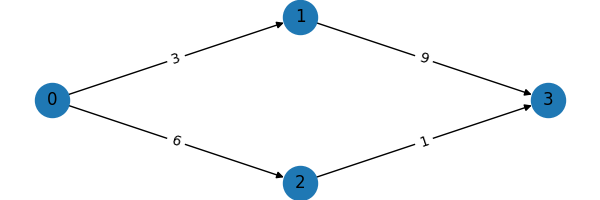
\includegraphics[scale=0.75]{zhiqiang-grafo/zhiqiang-grafo.png}
\end{figure}

Este grafo (\textit{fig.~\ref{fig:4-zhiqiang_grafo}}) tiene la misma cantidad de nodos que el grafo anterior (\textit{fig.~\ref{fig:4-primer_grafo}}) y una arista menos.
Esto se traduce en una aplicación de QAOA con menos restricciones pero con los mismos qubits.
\\
Con esta diferenciación se pretende estudiar el comportamiento de estos problemas al aumentar el número de capas.

\begin{itemize}
\item \textbf{Objetivo:}

  \begin{align}
    &\min(3X_{01} + 6X_{02} + 9X_{13} + 1X_{23}) \\
    &\textnormal{donde } X_{ij} = \begin{cases} \nonumber
      1 \textnormal{ si el camino contiene la arista del nodo \textit{i} al \textit{j}} \\
      0 \textnormal{ en otro caso}
    \end{cases}
  \end{align}

\item \textbf{Restricciones:}

  \begin{enumerate}
  \item $X_{01} + X_{02} = 1$: Equivalente a la \textit{restricción~\ref{it:4-primer_grafo_restriccion_ini}} del problema previo.

  \item $X_{01} = X_{13} \\
    X_{02} = X_{23}$: Equivalentes a las \textit{restricciones~\ref{it:4-primer_grafo_restriccion_inter}} del problema previo.

  \item $X_{13} + X_{23} = 1$:  Una restricción extra, similar a la primera.
    Debe haber exactamente un eje del camino que involucre al nodo final.
    Fuerza a que el camino finalice en dicho nodo

  \end{enumerate}

  Con el fin de mantener las similitudes con el problema anterior se elige el modificador de Lagrange (\textit{P}) utilizando la misma métrica, a saber:

  \begin{align}
    P = 1 + \max_{x}{(f_{\textnormal{sin restricc}}(x))} = 1 + \sum_{(i, j)\in{E}}{w_{ij}} = 20
  \end{align}

\end{itemize}

Al añadir las restricciones, como se explica en la \textit{sección~\ref{sec:3-problemas de optimizacion combinatoria}}, la función de coste definitiva en formato QUBO queda como:

\begin{align}
  f(X) &= 3X_{01} + 6X_{02} + 9X_{13} + 1X_{23} + \nonumber \\
       &+ P{(X_{01} + X_{02} - 1)}^2 + P{(X_{13} + X_{23} - 1)}^2 + P{(X_{01} - X_{13})}^2 + P{(X_{02} - X_{23})}^2
\end{align}

El desarrollo para obtener el hamiltoniano del problema, realizado con el mismo procedimiento que los problemas anteriores, se encuentra en la \textit{sección~\ref{CAP:DESARROLLO_ZHIQIANG_ISING}} del apéndice
\\
El hamiltoniano del problema (descrito en la \textit{sección~\ref{sec:3-circuito de qaoa}}) partiendo de $f(X)$ es:

\begin{align}
  &U(C, \gamma) = \exp(-i \gamma C) = \nonumber \\
  &= Rz_0(-1.5 * 2\gamma) \cdot Rz_1(-3 * 2\gamma) \cdot Rz_2(-4.5 * 2\gamma) \cdot Rz_3(-0.5 * 2\gamma) \cdot \nonumber \\
  &\cdot Rz_0z_1(10 * 2\gamma) \cdot Rz_0z_2(-10 * 2\gamma) \cdot Rz_1z_3(-10 * 2\gamma) \cdot Rz_2z_3(10 * 2\gamma)
\end{align}

Con el \textit{hamiltoniano de mezcla} y el vector inicial, definidos en la \textit{sección~\ref{sec:3-circuito de qaoa}} y el \textbf{hamiltoniano del problema} obtenido se puede construir el circuito cuántico.

\paragraph{Discusión de la diferencia entre circuitos de distintas implementaciones de QAOA}

\begin{figure}[Circuito {--} shortest path de Fan et al. (2023) propio]{fig:4-zhiqiang_circuito}{ Circuito obtenido con la implementación de QAOA del TFG ($p=1$) }
  \centering
  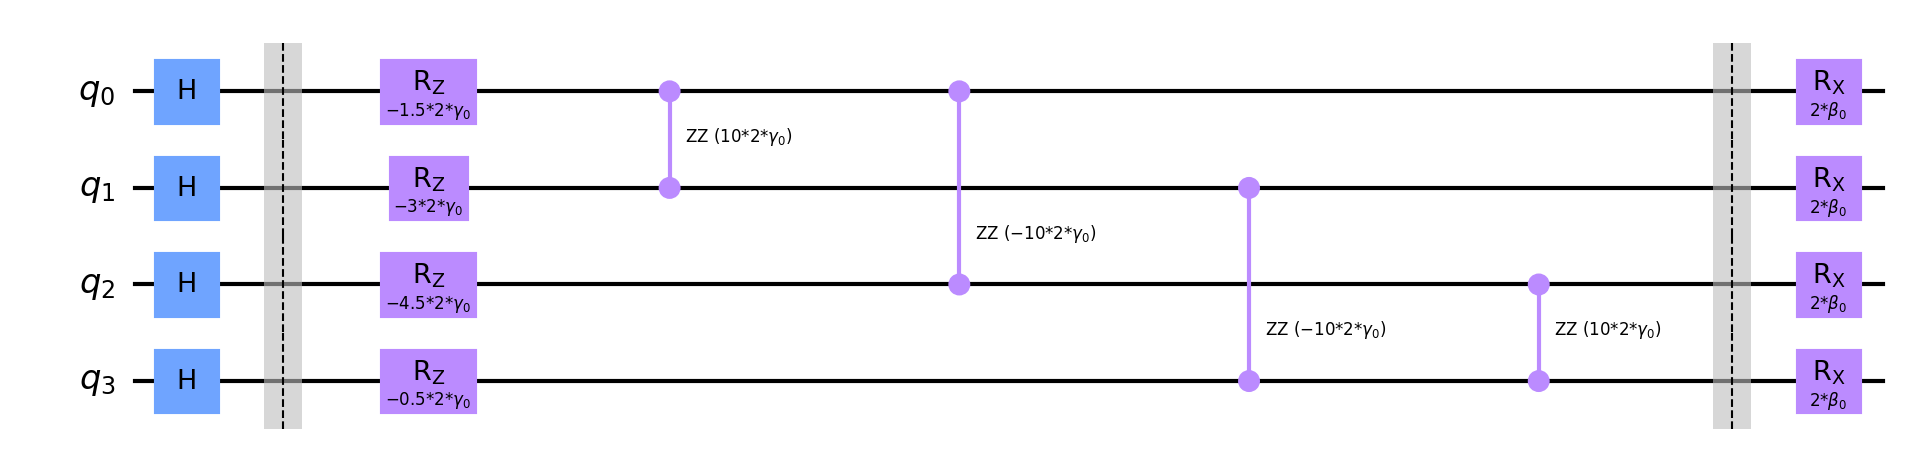
\includegraphics[scale=0.4]{circuits/zhiqiang/zhiqiang-circuit-p1-var.png}
\end{figure}

\begin{figure}[Circuito {--} shortest path de Fan et al. (2023) de QAOAAnsatz]{fig:4-zhiqiang_QAOAAnsatz_circuito}{ Circuito generado por QAOAAnsatz ($p=1$) }
  \centering
  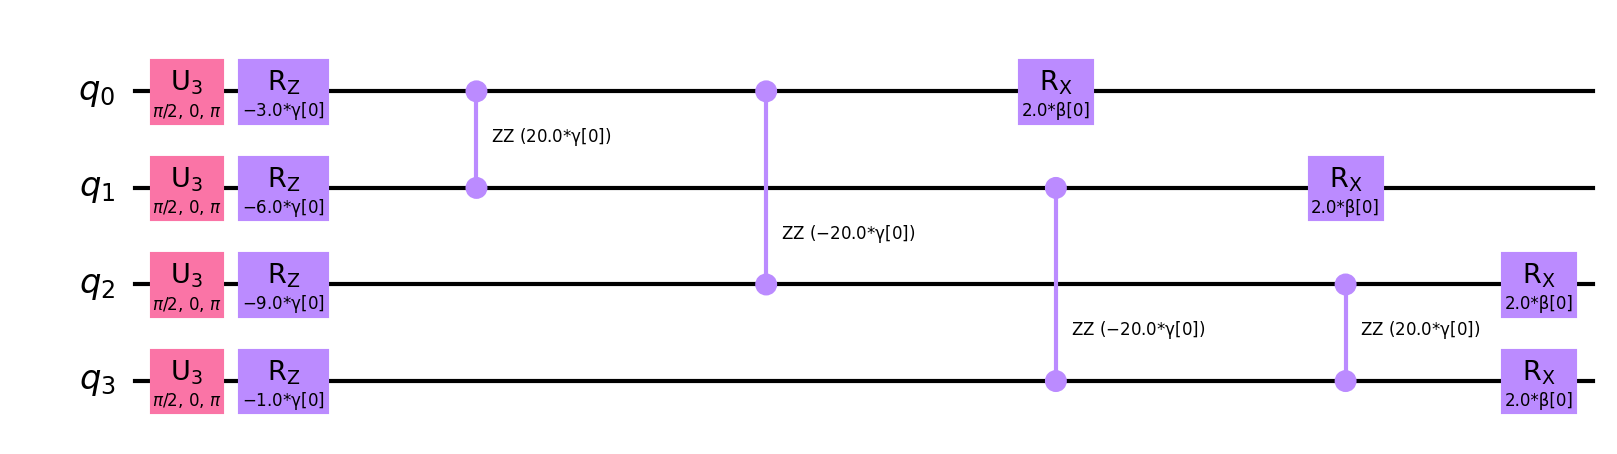
\includegraphics[scale=0.45]{circuits/zhiqiang/zhiqiang-circuit-qaoaAnsatz-p1.png}
\end{figure}

En el artículo por Fan et al. (2023)\cite{solving_shortest_path_with_qaoa}, del que se ha obtenido el problema, no se muestra la construcción del circuito de QAOA, por lo que el resultado obtenido en la \textit{fig.~\ref{fig:4-zhiqiang_circuito}} solo puede ser comparado con el circuito generado por la función \textit{QAOAAnsatz()} (fig.~\ref{fig:4-zhiqiang_QAOAAnsatz_circuito}).
\\
Como los circuitos son equivalentes se asume que la implementación del circuito parametrizado es correcta.


%%% Local Variables:
%%% mode: latex
%%% TeX-master: "../tfgtfmthesisuam"
%%% End:
